\newpage
\section{Hyperband}
Hyperband is an hyper-parameter optimization method invented by Li, Lisha, and Kevin Jamieson \cite{li2016novel}.
It was formulated as a pure-exploration nonstochastic infinite-armed bandit problem where a predefined resource like iterations, data samples, or features is allocated to randomly sampled configurations.\\

Hyperband extends the Successive Halving algorithm proposed for hyper-parameter optimization by Jamieson and Talwalkar \cite{jamieson2016non}. 

\begin{figure}[ht]
\centering
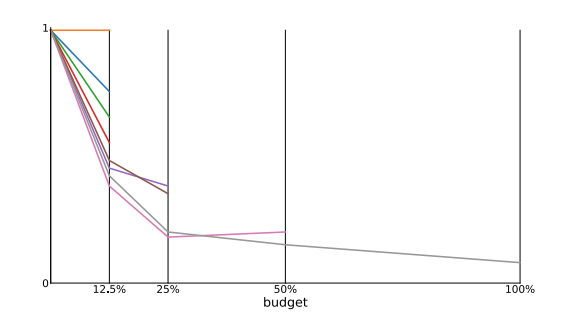
\includegraphics[scale=0.6]{images/Successive Halving.png}
\caption{Successive Halving example.}
\label{fig:Successive_Halving}
\end{figure}

The idea behind the original Successive Halving algorithm its about uniformly
allocate a budget to a set of hyper-parameter configurations, evaluate the performance of
all configurations, throw out the worst half, and repeat until one configuration remains.
The algorithm allocates exponentially more resources to more promising configurations \cite{li2016novel}\cite{jamieson2016non}.
Unfortunately, Successive Halving requires the number of configurations n and some finite budget B as inputs
to the algorithm. Than B/n resources are allocated on average across the configurations. 

However, in many cases it's not known if it's better to consider many configurations (large n) with a small average training time or consider a small number of configurations (small n) with longer average training times. \\ 

Hyperband requires two inputs: R, the maximum amount of resource that can
be allocated to a single configuration, and \(\eta\),that controls the proportion of
configurations discarded in each round of Successive Halving \cite{li2016novel}.

It tries to solve the problem by running several Successive Halving runs with different budgets and number of configurations, to find the best set.

Hyperband set  \( s_{max} = \lfloor \log_\eta B \rfloor \). It than begins with the most aggressive 
bracket \(s = s_{max}\), which sets n to maximize exploration. 
Each subsequent bracket reduces n by a factor of \(\eta\) until the final bracket, s = 0, in which every configuration is allocated R resources (this bracket simply performs classical random search). 
Hence, Hyperband performs a geometric search in the average budget per configuration and removes the need
to select n for a fixed budget at the cost of approximately \(s_max + 1\) times more work than
running Successive Halving for a single value of n. 
By doing so, Hyperband is able to exploit situations in which adaptive allocation works well, while protecting itself in situations where more conservative allocations are required \cite{li2016novel}.
